%% Trigonometrie III
%% Arkusfunktionen
%% 2020 - 12 - 21 φ@bbw.ch

\section{Arkusfunktionen}\index{Arkusfunktionen}

Einstiegsüberlegung: Von einem Winkel $\varphi$ ist gerade einmal sein Sinuswert bekannt: $0.6 = \sin(\varphi)$. Wie groß ist der Winkel?

\trigsysDsin{}


\TNT{6.4}{Hier gibt es unendlich viele Lösungen. Im Bereich 0 bis 90$\degre$ sind es jedoch genau zwei Lösungen: 1. Lösung: $\varphi=\arcsin(0.6) \approx 36.87$ und 2. Lösung: $\varphi = 180\degre - \arcsin(0.6) \approx{} 143.13$}

Mit dem Taschenrechner haben Sie zwei Varianten diesen Winkel zu berechnen:

A) \texttt{arcsin(0.6)}

B) \texttt{solve(0.6=sin(x), x)}

Was fällt Ihnen bei den Löusngen auf?
\newpage



\subsection{Arcussinus}
Auch die Umkehrungen der Sinus-, Cosinus- und Tangensbeziehungen können
als Funktionen aufgefasst werden.

Berechnen Sie von einigen \textbf{characteristischen}
ArcSin-Verhältnissen den zugehörigen Winkel und tragen Sie die Werte ins folgende
Koordinatensystem im Bogenmaß ein:

\begin{tabular}{l|c|r}
$\sin(0\degre)$ &=& $\LoesungsRaum{0}$\\\hline
$\sin(\LoesungsRaum{30\degre})$ &=& $\LoesungsRaum{0.5}$\\\hline
$\sin(\LoesungsRaum{45\degre})$ &=& $\LoesungsRaum{\frac{\sqrt{2}}{2}}$\\\hline
$\sin(\LoesungsRaum{60\degre})$ &=& $\LoesungsRaum{\frac{\sqrt{3}}{2}}$\\\hline
$\sin(\LoesungsRaum{90\degre})$ &=& $\LoesungsRaum{\frac{\sqrt{4}}{2} = 1}$\\\hline
$\sin(\LoesungsRaum{-30\degre})$ &=& $\LoesungsRaum{-0.5}$
\end{tabular}

\noTRAINER{\bbwCenterGraphic{8cm}{tals/trig3/img/py_system.png}}
\TRAINER{\bbwCenterGraphic{8cm}{tals/trig3/img/arcsin.png}}

Geben Sie den Definitionsbereich der Arcus-Sinus-Funktion an:

$$\mathbb{D} = \LoesungsRaum{\left[-1; 1\right]}$$

Geben Sie den Wertebereich der Arcus-Sinus-Funktion einmal im Bogenmaß,
einmal im Gradmaß an:
$$\mathbb{W} = \LoesungsRaum{\left[-\frac{\pi}{2}; \frac{\pi}{2}\right]}  =  \LoesungsRaum{[-90\degre; 90\degre]}$$
\newpage


\subsection*{Aufgaben}

Im Geometrie-Buch; doch diesmal anhand der Funktionsgraphen und nicht (nur) am Einheitskreis.

Vorzeigeaufgabe: Für welche(n) Winkel $\varphi$ gilt \fbox{$\sin(\varphi) = -\sin(-41.7\degre)$}?

\TRAINER{Lösung: $\varphi = 41.7\degre$ und $180\degre-41.7\degre=139.3\degre$ und alle periodischen Vielfachen: $\varphi\pm n\cdot{}360\degre$}

\trigsysDsin{}

Mit Taschenrechner:

\TALSGeomAadB{102ff}{85. a) c)}

Ohne Taschenrechner\footnote{Für die Grundlagenfachprüfung müssen Sie solche Aufgaben lösen können}:

\TALSGeomAadB{102ff}{85. e) f) g) und h)}


\newpage

\subsection{Arccuscosinus}
Zeichnen Sie die Umkehrfunktion des Cosinus und geben Sie den Definitionsbereich an.

\noTRAINER{\bbwCenterGraphic{8cm}{tals/trig3/img/py_system.png}}
\TRAINER{\bbwCenterGraphic{8cm}{tals/trig3/img/arccos.png}}


$$\mathbb{D} = \LoesungsRaum{[-1; 1]}$$

Geben Sie den Wertebereich der Arcus-Sinus-Funktion einmal im Bogenmaß,
einmal im Gradmaß an:
$$\mathbb{W} = \LoesungsRaum{[0; \pi]}  =  \LoesungsRaum{[0; 180\degre]}$$

\subsection*{Aufgaben}
Mit Taschenrechner:
\TALSGeomAadB{102ff}{86. b)}
Ohne Taschenrechner:
\TALSGeomAadB{102ff}{86. c) und e)}


\newpage


\subsection{Arcustangens}
Zeichnen Sie die Umkehrfunktion des Tangens (im Bogenmaß) und geben Sie den Definitionsbereich an.

\noTRAINER{\bbwCenterGraphic{8cm}{tals/trig3/img/py_system.png}}
\TRAINER{\bbwCenterGraphic{8cm}{tals/trig3/img/arctan.png}}


$$\mathbb{D} = \LoesungsRaum{\mathbb{R}}$$

Geben Sie den Wertebereich der Arcus-Sinus-Funktion einmal im Bogenmaß,
einmal im Gradmaß an:
$$\mathbb{W} = \LoesungsRaum{\left]-\frac{\pi}{2}; \frac{\pi}{2}\right[}  = \LoesungsRaum{\left]-90\degre; 90\degre\right[}$$

Beachten Sie, dass im Wertebereich $\mathbb{W}$ die Grenzen ($-90\degre$und $+90\degre$) nicht enthalten sind. Warum ist das so?

\subsection*{Aufgaben}
Mit Taschenrechner:
\TALSGeomAadB{102ff}{87. a)}
Ohne Taschenrechner:
\TALSGeomAadB{102ff}{87. c)}
\newpage


\subsubsection{Für Applikationsentwickler\LoesungsRaum{\,($\mathrm{atan2}()$)}}

Wir betrachten ein kleines Computerspiel, bei dem von einer
Abschussrampe im Punkt $O=(0|0)$ in einem Winkel $\varphi$ ein Geschoss
abgeschossen wird (siehe folgende beiden Graphiken). Die Längen sind
in Einheiten von \texttt{px}\footnote{Ein \texttt{px} ist ein
  sog. \textit{picture element} und ist ursprünglich die kleinste adressierbare
  Einheit auf dem Computerdisplay.} gegeben.

\begin{tabular}{p{11cm}c}
\textbf{Problem I}: Gegeben ist ein Winkel von $107\degre$ von der
Abschussrampe aus gesehen und gesucht sind die Koordinaten des Punktes
$P=(x_P|y_P)$, der in der Entfernung von 350 [px].
&
\raisebox{-4cm}{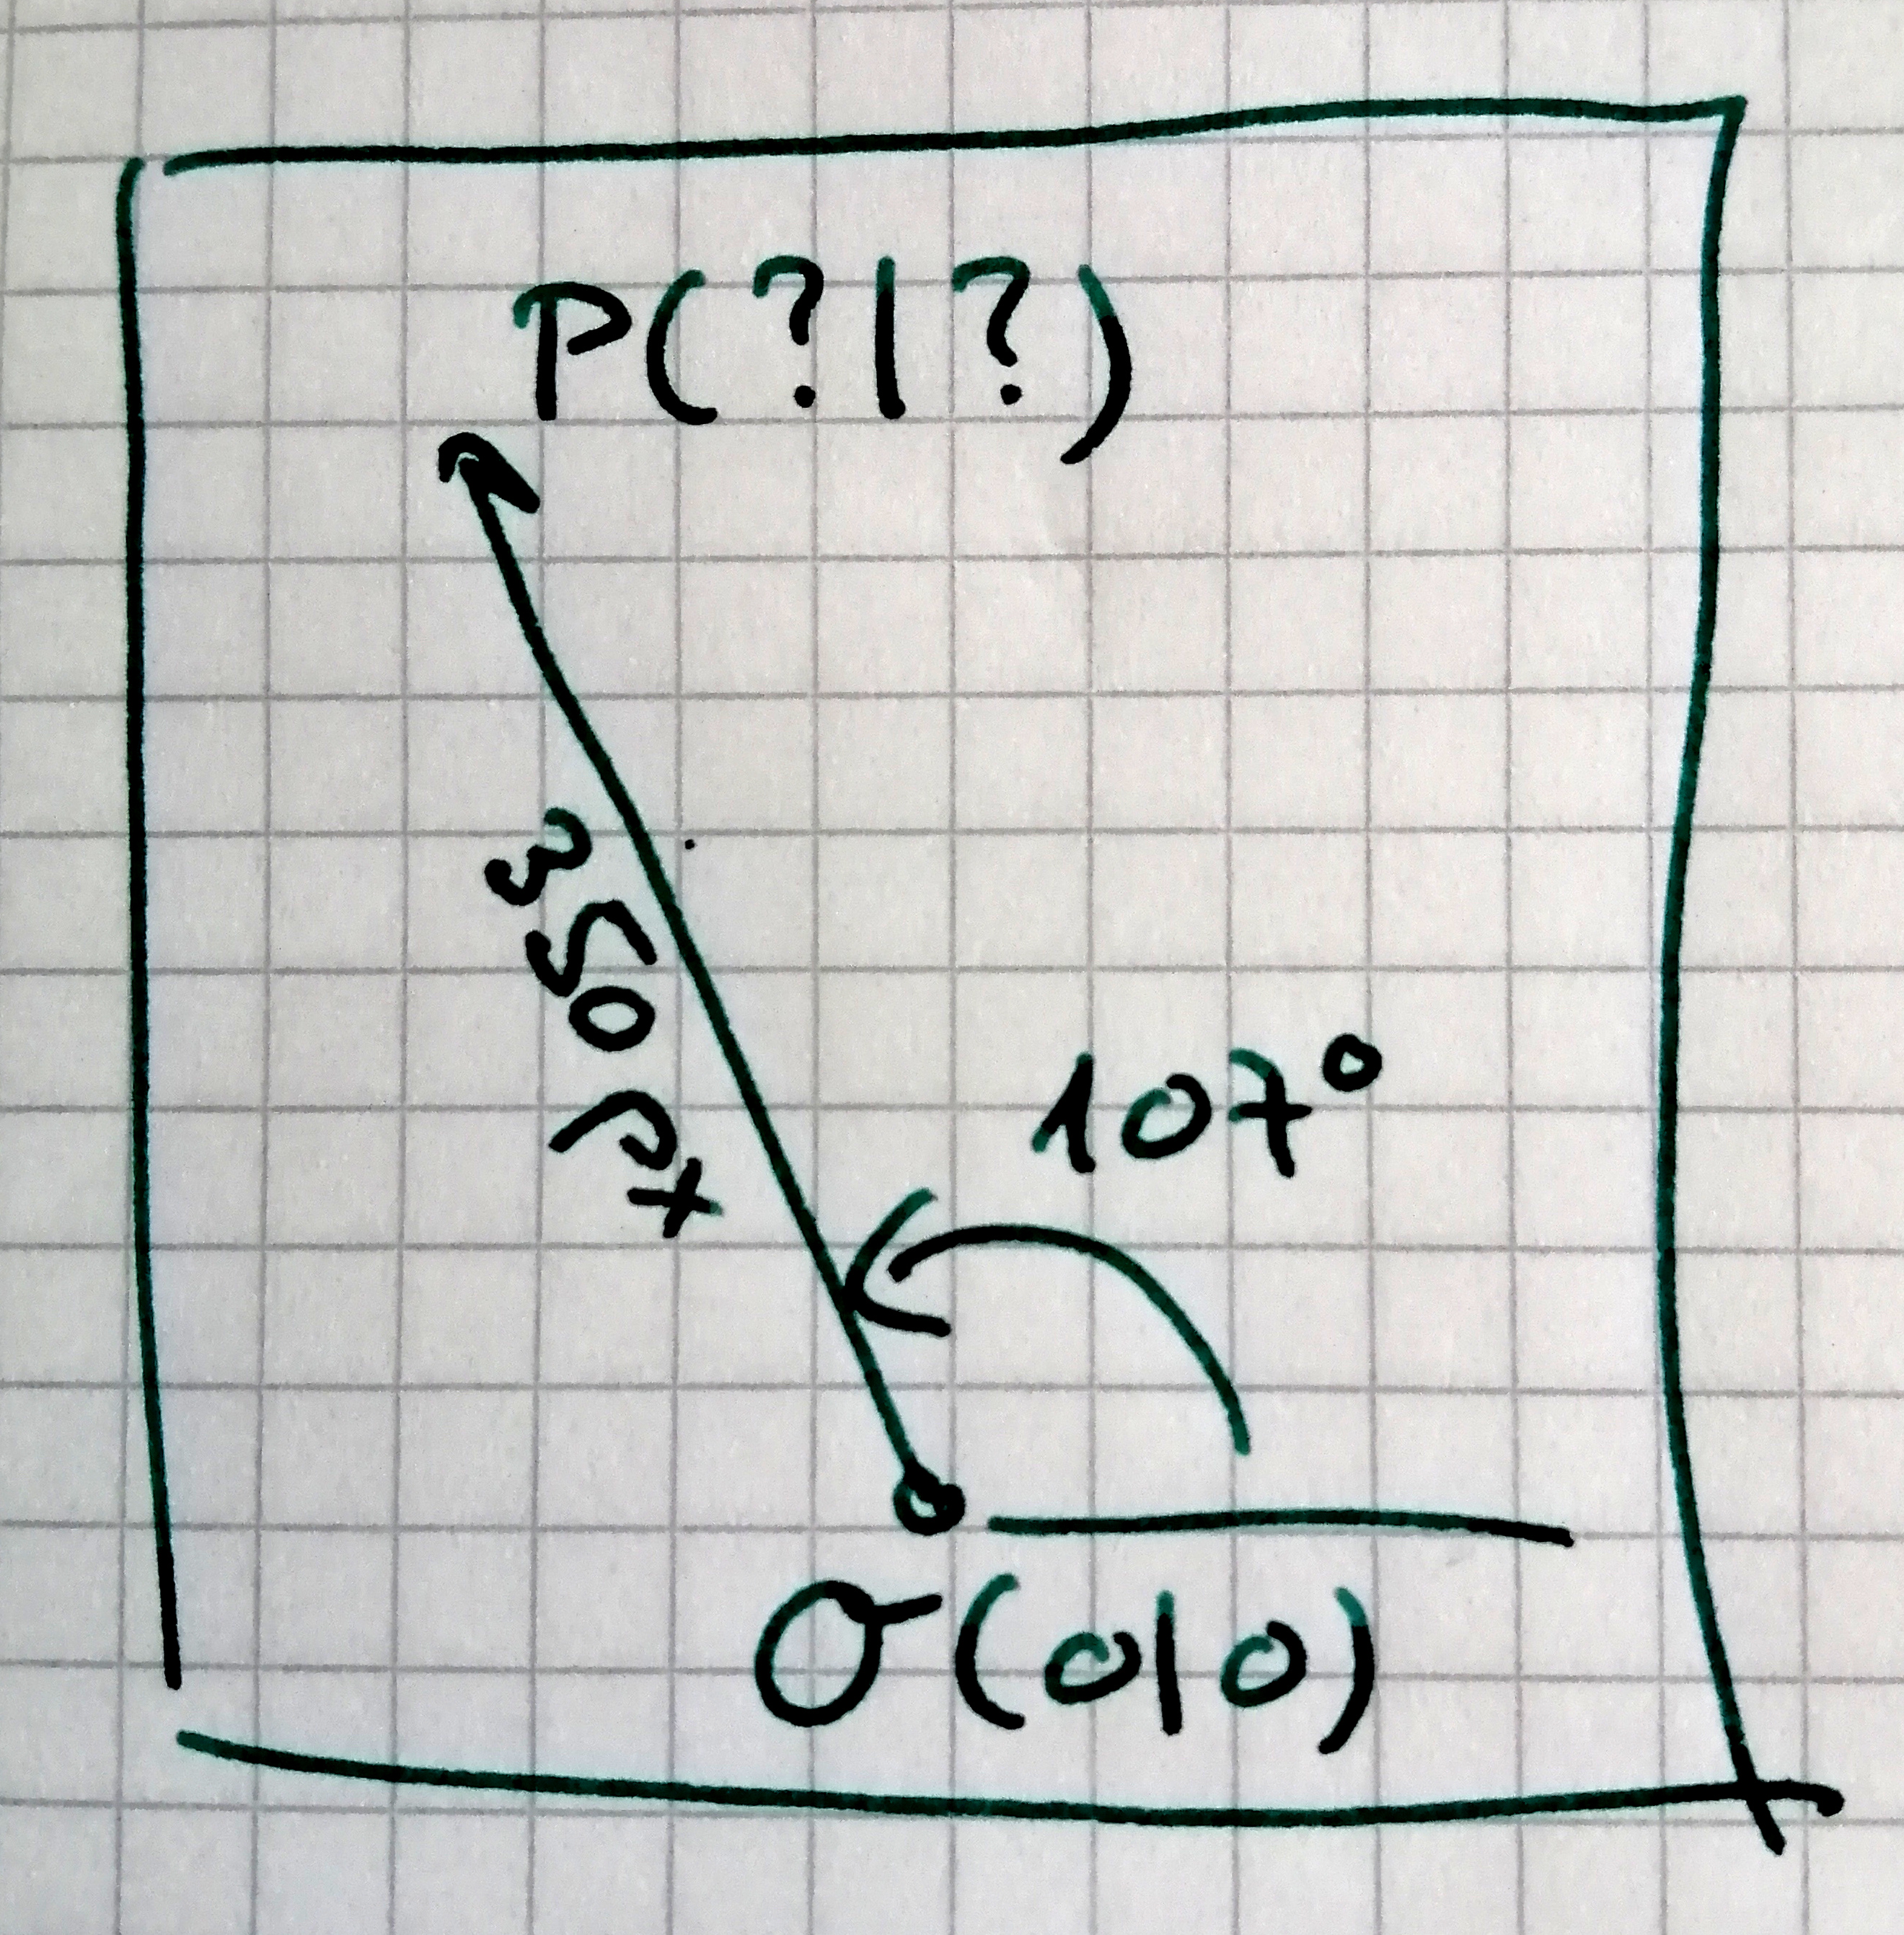
\includegraphics[width=5cm]{tals/trig3/img/atan2PunktGesucht.jpg}}\\
\end{tabular}

Lösung: $P=( \LoesungsRaumLang{350[px]\cdot{}\cos(107\degre)\approx{}-102[px]} | \LoesungsRaumLang{350[px]\cdot{}\sin(107\degre)\approx{}335[px]})$


\begin{tabular}{p{11cm}c}
\textbf{Problem II}: Gegeben ist neben dem Ursprung $O = (0 | 0)$ ein
weiterer Punkt $P=(x_P|y_P)$. In welchem Winkel $\varphi$ befindet sich
$P$ von $O$ aus gesehen? Gesucht ist der Winkel $\varphi$ im
mathematisch positiven Sinne.

&
\raisebox{-4cm}{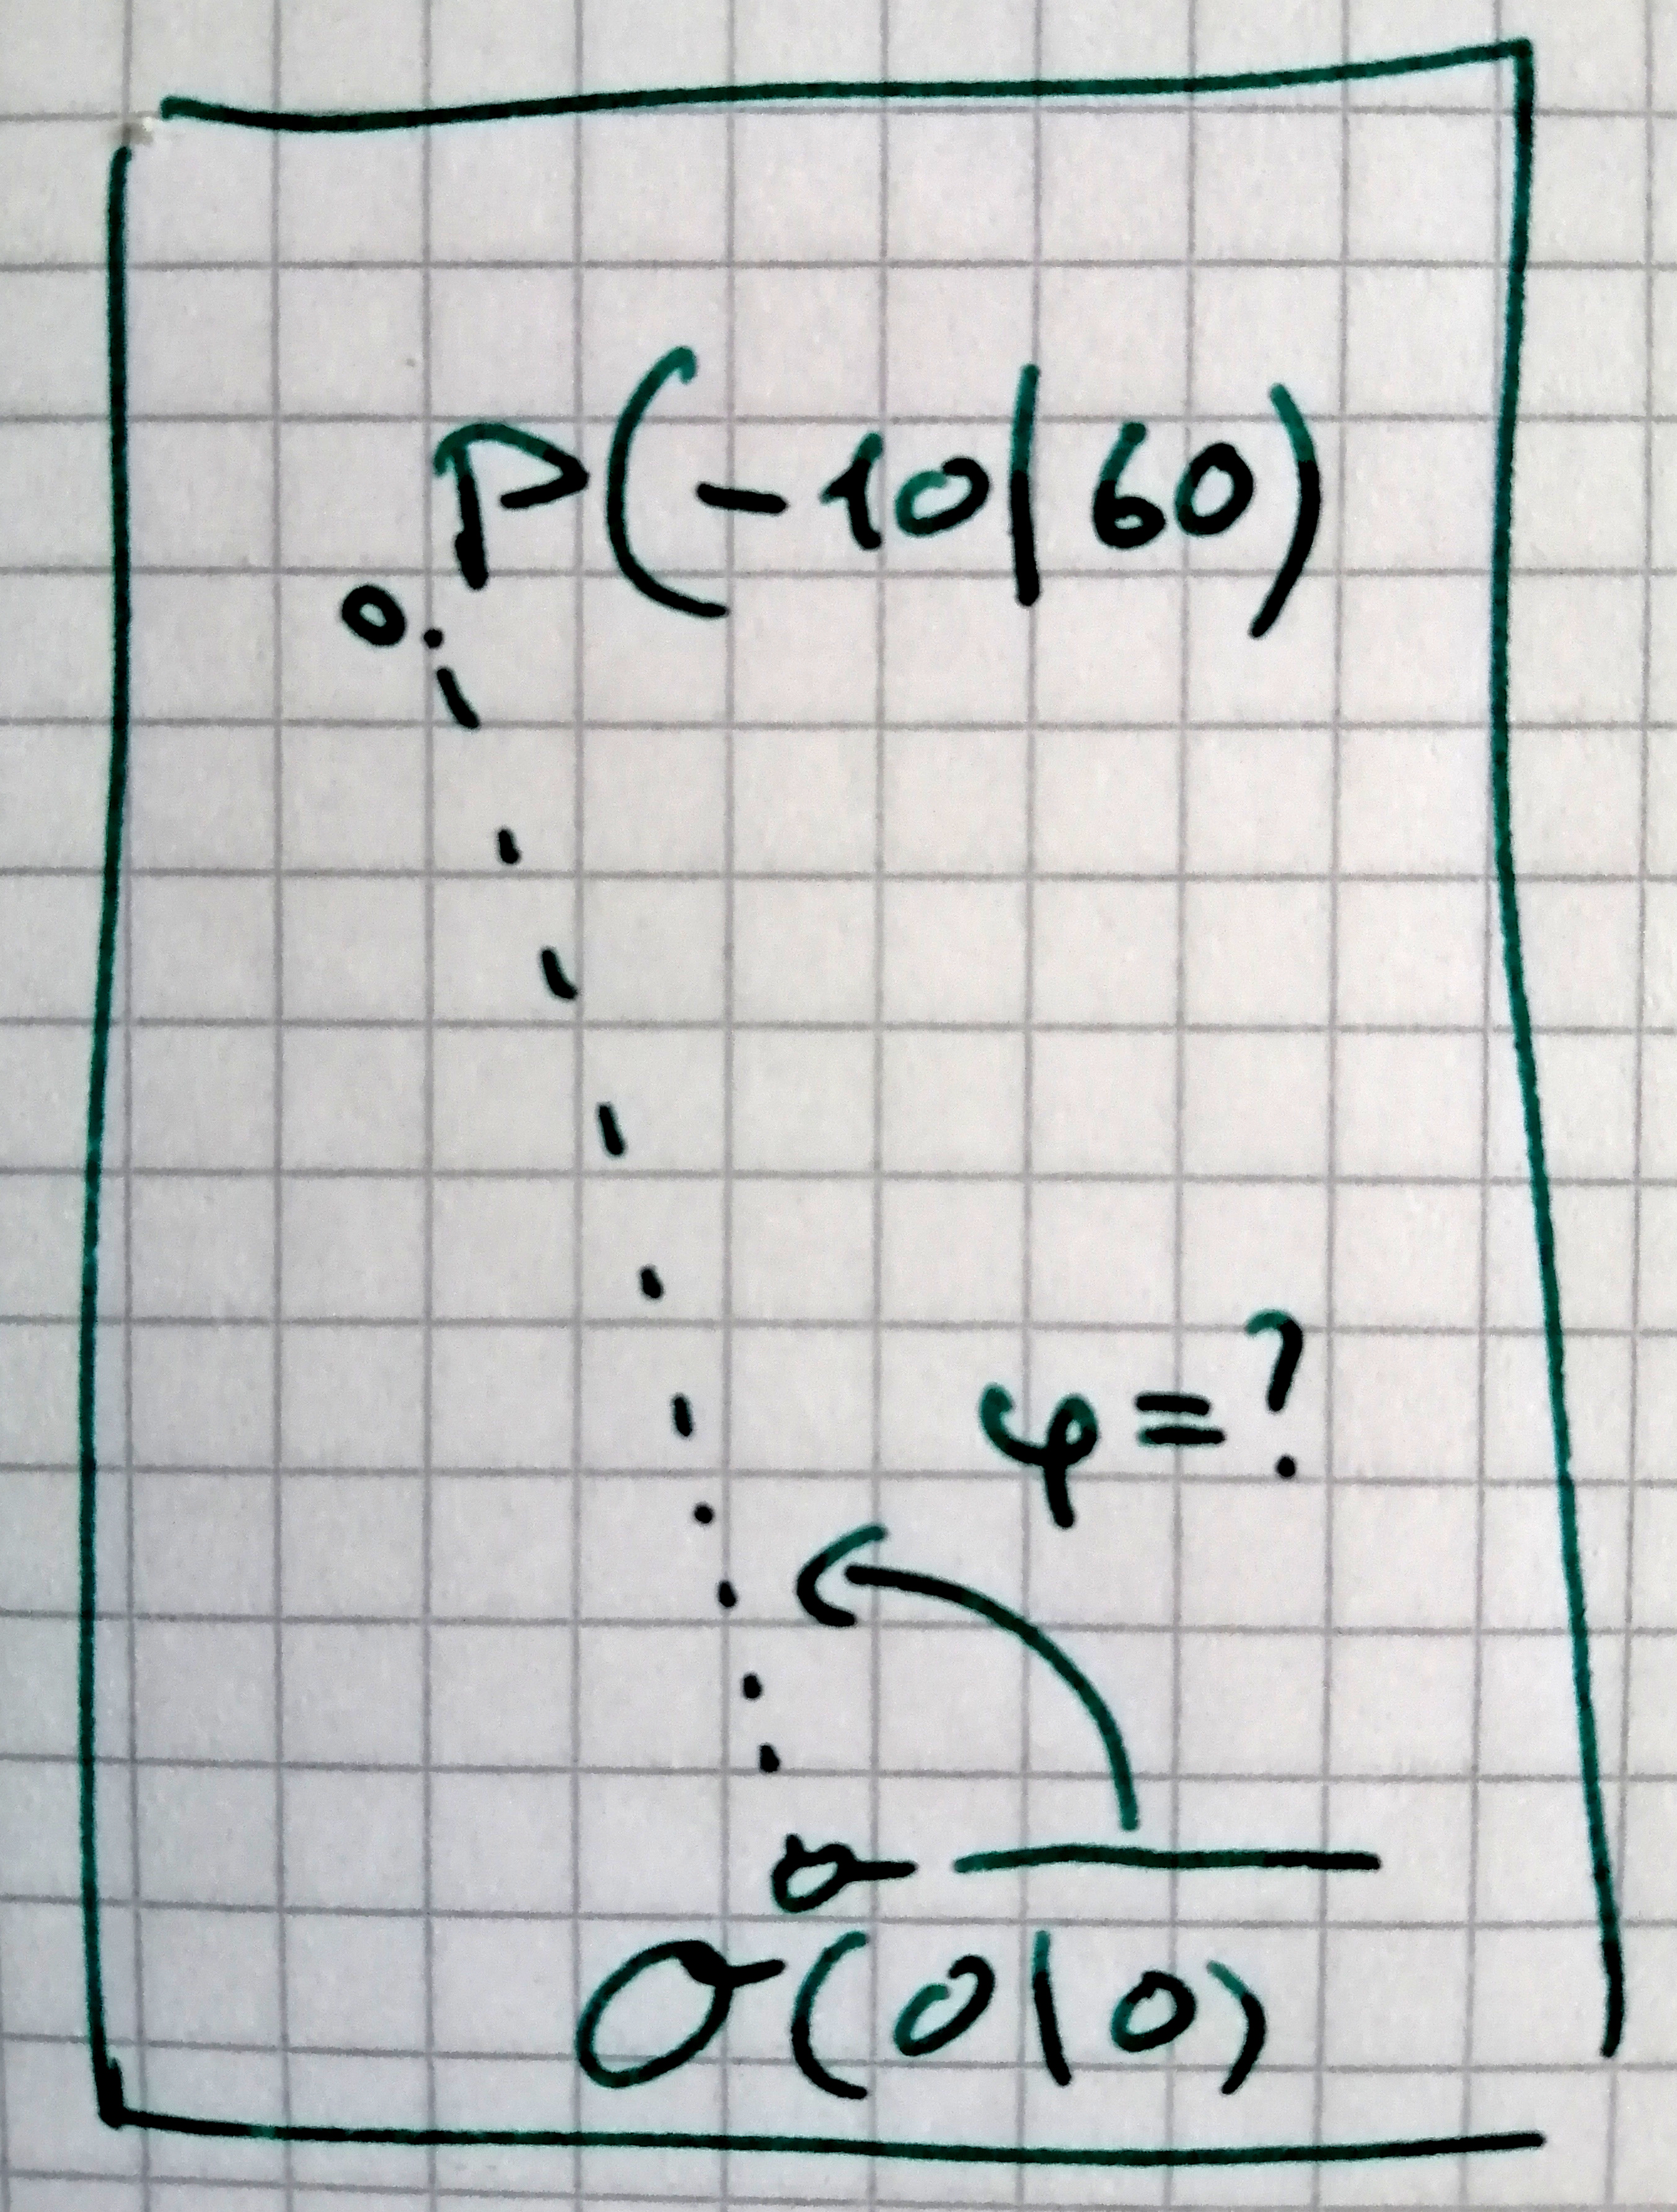
\includegraphics[width=5cm]{tals/trig3/img/atan2WinkelGesucht.jpg}}\\
\end{tabular}

Beispiele und Lösung:

\begin{tabular}{l|l|l}
  Punkt          & Winkel                  & allgemeine Formel? \\ \hline
  $P=(+10 |  60)$ & $\varphi = \LoesungsRaum{80.5\degre}$  & $\varphi=\LoesungsRaum{\arctan(\frac{y}{x})}$ \\ \hline
  $P=(-10 |  60)$ & $\varphi = \LoesungsRaum{99.46\degre}$ & $\varphi=\LoesungsRaum{90\degre - \arctan(\frac{y}{x})}$ \\ \hline
  $P=(  0 |  70)$ & $\varphi = \LoesungsRaum{90\degre}$    & $\varphi=$\LoesungsRaum{Sonderfall, sonst Division durch 0} \\ \hline
  $P=(-20 |   0)$ & $\varphi = \LoesungsRaum{180\degre}$   & $\varphi=\LoesungsRaum{\arctan(\frac{y}{x}) + 180\degre}$ \\ \hline
  $P=(x_P | y_P)$ & allgemeiner Fall?      & $\varphi=\LoesungsRaum{\textrm{\textbf{atan2}}(\textbf{y}, \textbf{x})}$\\ \hline
\end{tabular}

\TNT{2.8}{
Beispiel unter \texttt{html-css-js.com}: im HTML-Fenster: \texttt{<p
  id='test'/>} und im javascript-Fenster:

\texttt{document.getElementById('test').innerHTML = 180 * Math.atan2(10, 5) / Math.PI;}%%
}%% END TNT
